\documentclass[conf]{new-aiaa}
%\documentclass[journal]{new-aiaa} for journal papers
\usepackage[utf8]{inputenc}

\usepackage{graphicx}
\usepackage{amsmath}
\usepackage[version=4]{mhchem}
\usepackage{siunitx}
\usepackage{longtable,tabularx}
\usepackage{float}
\usepackage{subfigmat}
\usepackage{setspace}
%\doublespacing

\floatstyle{boxed}
\restylefloat{figure}

\setlength\LTleft{0pt} 

\title{Vector field  path following and obstacle avoidance singularity mitigation via look-ahead flight envelope}

\author{First A. Author\footnote{Insert Job Title, Department Name, Address/Mail Stop, and AIAA Member Grade (if any) for first author.} and Second B. Author Jr.\footnote{Insert Job Title, Department Name, Address/Mail Stop, and AIAA Member Grade (if any) for second author.}}
\affil{Business or Academic Affiliation 1, City, State, Zip Code}
\author{Third C. Author\footnote{Insert Job Title, Department Name, Address/Mail Stop, and AIAA Member Grade (if any) for third author.}}


\begin{document}

\maketitle

\begin{abstract}



Unmanned Aerial Vehicles conventionally navigate by following a series of pre-planned waypoints that may have to be re-planned when flying in a dynamic environment or encountering previously unknown obstacles. Waypoints are generally planned off-line and relayed to the UAV, taking up time and autopilot communication resources. Attractive path following and repulsive obstacle avoidance vector fields have been summed together to produce UAV guidance that follows pre-planned paths and avoids obstacles without the need to re-plan. Summing attractive and repulsive vector fields may produce small regions of null guidance, called singularities, which could potentially lead to trap situations. An investigation into singularity mitigation by vector field weight parameterization is presented. 


\end{abstract}



\section{Nomenclature}

{\renewcommand\arraystretch{1.0}
\noindent\begin{longtable*}{@{}l @{\quad=\quad} l@{}}
$UAV$  & Unmanned Aerial Vehicle \\
$VF$   & Vector Field \\
$VFF$  & Virtual Force Field \\
$LVF$  & Lyapunov Vector Field \\
$GVF$  & Goncalves Vector Field \\
\end{longtable*}}

\section{Introduction}


%Paths have already been deemed to meet mission requirements
%Avoiding obstacles while minimizing deviation from the prescribed path would be benefitial
%Planning missions (path connecting sequential tasks)
%Following path with waypoints
%
%
%There are many methods for planning obstacle free and flyable paths, however in general the methods can be simplified into two steps consisting of optimization and path refinement. Optimization determines the least cost straight line path which is further refined to ensure the path is flyable.
%
%INTRODUCTION TO UAVS

Unmanned Aerial Vehicles (UAV)s are pilotless aircraft used by military, police, and civilian communities for tasks such as reconnaissance, damage assessment, surveying, and target tracking \cite{ariyur_autonomous_2008,teuliere_chasing_2011}. Tasks can be performed by a single UAV or cooperate with a team of other air, ground, or marine vehicles \cite{oh_coordinated_2013,hyondong_oh_coordinated_2015,ulun_coordinated_2013}. UAVs are ideal for remote data collection due to their low cost, endurance, and reduced risk to human life. Data can be collected by loitering the aircraft around an area of interest (AOI) or along a sensor path, such as a road or tree-line. Missions for collecting data are typically pre-planned on a remote ground station where an obstacle free and flyable path is generated. Constraints such as optimizing sensor converge may be considered when planning \cite{wilhelm_direct_2017}. Typically paths are deconstructed into a series of discrete waypoints that the UAV navigates to through the use of a line-of-sight guidance. While navigating the pre-planned path previously unknown obstacles may be discovered and a new obstacle free path may have to be generated, which may be difficult or impossible if the UAV is out of radio range. Directing the UAV to temporarily deviate from the planned path to avoid an obstacle may be accomplished with an on board guidance such as Potential Field or path following Vector Field. Potential field is a popular solution to both path planning and guidance problems in obstacle rich environments, however suffers from several limitations including local minima, oscillations, and may cause excess deviation from the desired sensor line. Vector field converges and circulates a pre-defined path and may be summed with additional repulsive vector fields to produce an obstacle avoidance guidance. Avoidance fields may be further optimized to reduce the deviation from a sensor path by modifying convergence and circulation scalar weights. Additionally, summing attractive and repulsive fields may result in singularities, small regions of null guidance that can produce trap situations. The contribution of this work is to provide an optimized vector field guidance for path following and obstacle avoidance as well as providing a method for identifying vector field singularities. First, the Dubin's UAV model will be presented followed by a description of waypoint guidance, potential field, and vector field. A method for singularity detection in summed vector field will be discussed, followed by a modified obstacle avoidance vector field. Simulations comparing the discussed guidance methods were conducted along with a multirotor demonstration of the improved vector field. 


\subsection{Dubins Vehicle}
UAVs traveling at constant altitude and velocity and with a limited turn rate can be simplified as a Dubin's vehicle that flies in straight line and circular arcs. It was assumed that an on-board controller accepts heading commands and produces vehicle roll to change the vehicles heading. The position $\overrightarrow{X}$ at time $t$ is calculated from the integral of the velocity vector $\overrightarrow{U}$. The vehicle has a constant velocity magnitude $u_{uav}$ at a heading $\theta$. Heading is an input from a guidance system, such as waypoint, potential field, or vector field.

\begin{equation}
\label{uavVelocity}
\overrightarrow{U}(t) = u_{uav} \begin{bmatrix}
cos(\theta(t)) \\
sin(\theta(t))
\end{bmatrix}
\end{equation}


\begin{equation}
\label{uavPosition}
\overrightarrow{X}(t) = \overrightarrow{U}dt + \overrightarrow{X}(t-1)
\end{equation}


\begin{equation}
\label{turnRate}
\dot{\theta} \leq 20 deg/s
\end{equation}



\subsection{Waypoint Guidance}
Waypoint guidance aligns the vehicle with the currently active waypoint that lies along a pre-planned path. Paths are typically generated off-line and can be optimized for shortest distance traveled and further refined to be flyable for a particular vehicle. Paths may also be optimized to produce flight patterns that increase sensor coverage of an area of interest \cite{wilhelm_direct_2017}. If an obstacle lies along that sensor path, the UAV must avoid the obstacle but also return back to the sensor path such that a minimal length of the path is missed during data collection. Waypoints placed on the outside the radius of the obstacle can direct a UAV around an obstacle and back onto the desired sensor path. Obstacles discovered during flight that lie along the pre-planned path may require a new path to be planned, requiring communication with the ground station. If a new path is not relayed to the UAV in time the vehicle may fail to avoid the obstacle. Additionally, if a new path is generated, it will most likely require that waypoints be placed some distance away from the obstacle's edge to accommodate the wayoints detection radius, increasing both deviation and time spent away from original path. An example of waypoints planned around an obstacle is shown in Figure \ref{fig:purewaypoint} below. 



%Typically the criteria for switching waypoints involves the UAV passing through a radius surround the current active waypoint. Due to the waypoint radius, waypoints may have to be placed further way from the obstacle to ensure the obstacle is not violated, causing the UAV to deviate and spend more time away from the sensor path. 
%
% A geometrically optimal path around a circular obstacle for a vehicle with fixed turn rate constraints can be generated in three steps. First, the UAV turns away from the obstacle such that it eventually becomes tangent to the obstacle radius. The vehicle then would proceed to follow the outside of the obstacle until nearly approaching the original sensor path. The UAV would then turn back towards the intended sensor path. An example of a series of waypoints that route a UAV with fixed wing constraints around an obstacle is shown in Figure \ref{fig:purewaypoint} below. 




%Generating a path to avoid an obstacle that lies on top of a sensor line can be constructed by considering the UAV turning radius and the radius of the obstacle.
%- Reconstruct path into discrete waypoints
%- Relay waypoints to a UAVs autopilot where guidance directs UAV towards waypoints
%- Planned at a ground station
%- Collision free path
%- Further optimized for vehicle constraints
%- Waypoints not optimal
%- Placed so radius is outside of obstacle
%- Generation is typically performed off-board
%- Communication with vehicle may not be possible
%- Obstacle avoidance may be achieved in the guidance system instead of path planning
% When collecting data it is important to stay as close to a prescribed path as possible to maximize sensor coverage of the area while avoiding collisions.
% 
% Obstacle free and flyable paths are typically pre-planned and generated off-line at a dedicated ground station using a path planner. 
% 
% Many methods can be used for generating paths, however the process is generally executed in two steps consisting of optimization and refinement. Optimization builds shortest path taking in constraints such as obstacles and mission objectives. 
% 
% The optimized path is then refined to meet a vehicles dynamic constraints, such as turn rate and velocity. UAVs using a line-of-sight guidance are sent a series of waypoints that lie along the pre-planned path over radio. The autopilot's guidance system directs the UAV to turn the crafts heading towards the current active waypoint, traveling in circular arcs and straight paths.  Curved sections of the refined path may require a dense spacing of waypoints to ensure the UAV tracks the refined path accurately. An example of a UAV following a series of waypoints that lie along a prescribed path is shown in Figure (). 

%
%\begin{figure}[H]
%	\centering
%	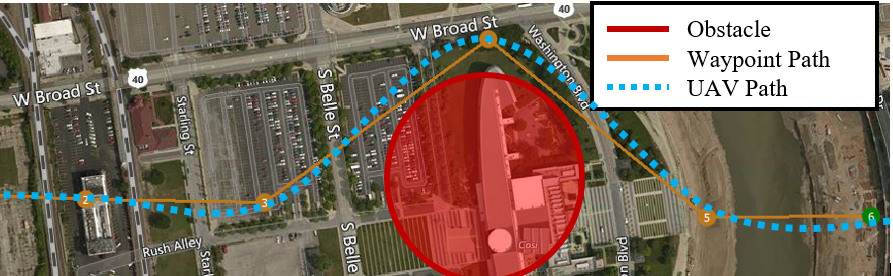
\includegraphics[width=1\linewidth]{Figures/simpleWaypointsWithUAVPath}
%	\caption{UAV path from waypoint guidance}
%	\label{fig:simplewaypointsWithUAVPath}
%\end{figure}

\begin{figure}[H]
	\centering
	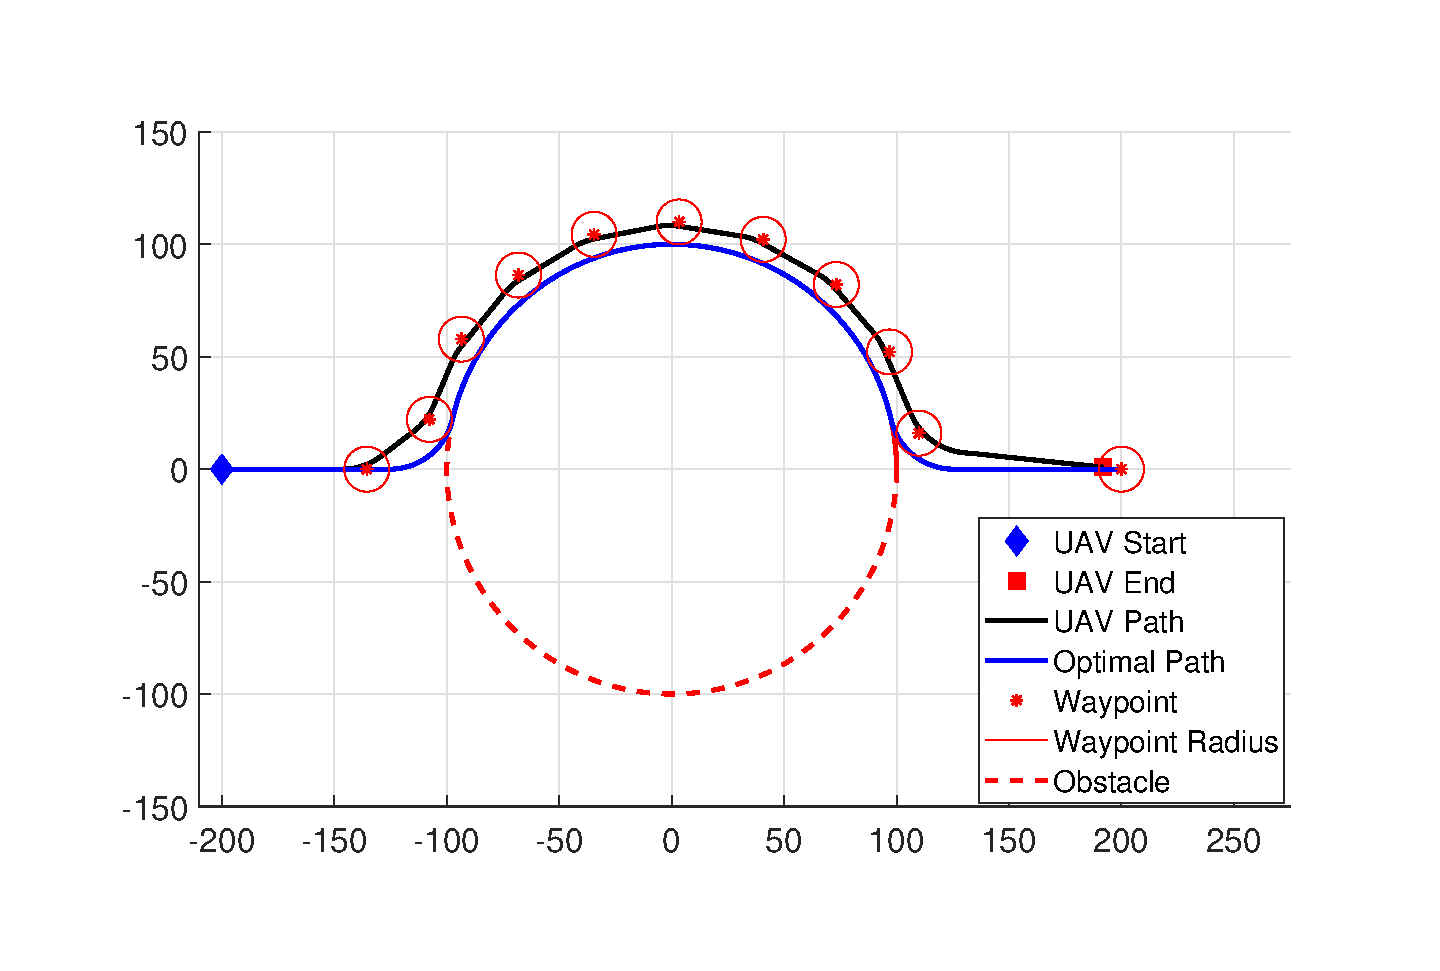
\includegraphics[width=0.7\linewidth]{Figures/Simulations/pureWaypoint}
	\caption{Simulated Fixed Wing UAV Traversing Waypoints Around Circular Obstacle}
	\label{fig:purewaypoint}
\end{figure}

It would be beneficial to include obstacle avoidance into a UAVs guidance system to remove the need to communicate with the ground station and path re-planning. 

%\section{Optimal Path}
%\begin{equation}\label{eq:optPath}
%y = \frac{u}{\dot{theta}} \newline
%\end{equation}
%
%\begin{equation}\label{eq:optPath}
%X = obstX - \sqrt{(turnR-obstR)^2-(y-obstY)^2}
%\end{equation}
%
%\begin{equation}\label{eq:optPath}
%\Theta = \sin^{-1}\Bigg(\frac{y-obstY}{obstR+turnR}\Bigg)
%\end{equation}
%
%\begin{equation}\label{eq:optPath}
%\beta = \Big[\frac{3\pi}{2},\pi-\Theta\Big]
%\end{equation}
%
%\begin{equation}\label{eq:optPath}
%\gamma = \Big[\pi-\Theta,\Theta\Big]
%\end{equation}
%
%\begin{equation}\label{eq:optPath}
%\zeta = \Big[\pi+\Theta,\frac{30pi}{2}\Big]
%\end{equation}
%
%\begin{equation}\label{eq:optPath}
%x = 
%\begin{cases} 
%0 & X+turnR*cos(beta) \\
%\frac{100-x}{100} & obstX + obstR*cos(gamma) \\
%0 & -X+turnR*cos(zeta) 
%\end{cases}
%\end{equation}



% For highly uncertain or dynamic environments, path planning may have to occur frequently which increases communication overhead for the autopilot
%
%% The state of the environment would then need to be transmitted back to the ground station and a new optimized and refined path be generated along with a series of waypoints. 
%%
%%
%%
%%During waypoint navigation the UAV may encounter obstacles or environmental changes that would require a new set of obstacle free waypoints to be generated. 
%
%
%For highly uncertain or dynamic environments, there may have to be frequent updates which increases the communication overhead of the autopilot since paths may be updated and communicated from the ground. Additionally, if communication is delayed or lost, waypoints may not be updated rapidly enough and the UAV may fail to avoid the obstacles if the autopilot is following outdated waypoints that violate an obstacle. Real time obstacle avoidance without the need to replan may be found in the use of potential and vector fields, which operate on the principle of artificial attractive and repulsive forces to guide a robotic system. 


\subsection{Potential Field}

Potential field is based on the principle of artificial attractive and repulsive forces acting on a point mass to guide a system to a desired goal while avoiding static and dynamic obstacles \cite{khatib_real-time_1986}. Goals states are represented as an attractive force that pulls a point mass in the direction of minimal energy while obstacles are represented as repulsive forces that act locally to push the point mass away. Potential field also is capable of acting as a path and trajectory planning algorithm \cite{rimon_exact_1992}, possibly eliminating the off-board path planner. An example of potential field can be found in \cite{borenstein_real-time_1990,borenstein_vector_1991,koren_potential_1991} which allowed for real time goal seeking with obstacle avoidance on a mobile ground robot equipped with ultrasonic sensors. The robot located at $(x_0,y_0)$ is attracted towards a a goal with constant magnitude force $\overrightarrow{F_t}$ located at $(x_t,y_t)$ and a distance $d_t$ from the robot. In the immediate area of the robot, an active window exists which records integer certainty values inside discrete cells. Cells containing an obstacle provide a repulsive force $\overrightarrow{F_{i,j}}$ opposite in direction to the line-of-sight from vehicle to cell location $(x_i,y_j)$, where $(i,j$) represents the cell index, $F_{cr}$ is a constant repulsive force, $W$ the vehicle's width, $C_{i,j}$ a cell's certainty, and $d_{i,j}$ the distance to the center of the cell with respect to robots center.

\begin{equation}\label{eq:vffRepulse}
\overrightarrow{F_{i,j}} = \frac{F_{cr}W^nC_{i,j}}{d^n_{i,j}} \bigg( \frac{x_i-x_0}{d_{i,j}}\hat{x} + \frac{y_i-y_0}{d_{i,j}}\hat{y}\bigg)
\end{equation}

The total repulsive force exerted on the robot is determined by summing the active cells, shown in Equation \ref{eq:vffRepulseSum}


\begin{equation}\label{eq:vffRepulseSum}
\overrightarrow{F_r} = \sum_{i,j}\overrightarrow{F_{i,j}}
\end{equation}


\begin{equation}\label{eq:vffGoal}
\overrightarrow{F_t} = F_{ct} \bigg( \frac{x_t-x_0}{d_{t}}\hat{x} + \frac{y_t-y_0}{d_{t}}\hat{y}\bigg)
\end{equation}

Summing together attractive and repulsive forces produce a vector that can be used for heading guidance, shown in Equation \ref{eq:vffHeading}.

\begin{equation}\label{eq:vffHeading}
\overrightarrow{R} = \overrightarrow{F_r} + \overrightarrow{F_t}
\end{equation}

 Major drawbacks to potential field were identified in \cite{koren_potential_1991} consisting of local minimum and oscillations in corridors. The local minimum problem occurs when closely spaced obstacle's potential combine to produce a well on the descent gradient where a pre-mature stable point is reached. Proposed solutions to local minimum include object clustering and virtual waypoint method \cite{liu_virtual-waypoint_2016}, virtual escaping route \cite{kim_escaping_2009}, and use of navigation functions \cite{goerzen_survey_2010}. Oscillations in potential field were studied in \cite{lei_tang_novel_2010} and \cite{li_efficient_2012}.


In addition to local minimum and oscillations, potential field may not be ideal for providing guidance to return to a sensor path after avoiding an obstacle. Once the obstacle has been avoided, the attractive goal will direct the UAV in a straight path which may not lie along the sensor line. Guidance that follows an explicit path, deviates when necessary to avoid obstacles, and returns back to the explicit path quickly can be accomplished with path following vector fields. 


\subsection{Vector Field Guidance}

 Vector fields produce continuous heading guidance that asymptotically converges and circulates a path. A comparison between vector field and waypoint guidance techniques was presented in \cite{sujit_unmanned_2014} where each method was evaluated based on its complexity, robustness, and accuracy. The vector field model produced guidance that was both robust to external wind disturbances while maintaining a low cross track error. The two most prominent methods for generating vector fields in literature consist of the Lyapunov \cite{nelson_cooperative_2005,nelson_vector_2006,nelson_vector_2007,frew_cooperative_2007,miao_orthogonal_2016,griffiths_vector_2006} and Goncalves \cite{goncalves_artificial_2009,goncalves_circulation_2010,goncalves_vector_2010,gerlach_autonomous_2014} method. Lyapunov vector fields for converging and following straight and circular paths were described in \cite{nelson_cooperative_2005}. Straight and circular path vector fields can be selectively activated throughout flight to form more complex paths, shown in \cite{nelson_cooperative_2005,nelson_vector_2006,nelson_vector_2007,jung_unmanned_2016}. Lyapunov vector field for curved path following was presented in \cite{griffiths_vector_2006} which may allow for more complex paths and eliminates the need to switch between vector fields. \\

\subsection{GVF}
The Gonvalves Vector Field (GVF) method produces a similar field, however has several advantages over LVFs. GVF produces an \textit{n}-dimensional vector field that converges and circulates to both static and time varying paths. Additionally, convergence, circulation, and time-varying terms that make up the GVF are decoupled from each other allowing for easy weighting of the total field. GVFs converge and circulate at the intersection, or level set, of $n-1$ dimensional implicit surfaces ($\alpha_i:\mathbb{R}^n\rightarrow\mathbb{R} | i=1,...,n-1$). The integral lines of the field are guaranteed to converge and circulate the level set when two conditions are met: $1)$ the implicit surface functions are positive definite and $2)$ have bounded derivatives. %Consider the space with dimensions in set \textbf{q}:

%The Goncalves Vector Field (GVF) method for producing vector fields has several advantages over the Lyapunov vector field generation methods.


%\begin{equation}
%\mathbf{q} = \begin{bmatrix} x_1, x_2, ..., x_{n}\end{bmatrix}
%\end{equation}

The total vector field $\overrightarrow{V}$ is calculated by:
\begin{equation}\label{eq:GVF}
\overrightarrow{V} = G \nabla V + H \wedge_{i=1}^{n-1}\nabla\alpha_i  - LM(\alpha)^{-1} a(\alpha)
\end{equation}

or in component form:

\begin{equation}\label{simpleGVF}
\overrightarrow{V} = G\overrightarrow{V}_{conv} + H\overrightarrow{V}_{circ} + L\overrightarrow{V}_{tv} 
\end{equation}	

where $\overrightarrow{V}_{conv}$ produces vectors perpendicular to the path, $\overrightarrow{V}_{circ}$ produces vectors parallel to the path, and $\overrightarrow{V}_{tv}$ is a feed-forward term that produces vectors accounting for a time varying path. 

Convergence is calculated by:

\begin{equation}
% Total field with Conv, Circ, and Time
\vec{V}_{conv} = \nabla V  
\label{convOnly}
\end{equation}


where scalar $G$ is multiplied by the gradient of the definite potential function $V$:

\begin{equation}
V = -\sqrt{{\alpha_1}^2 + {\alpha_2}^2}
\end{equation}

\begin{equation}
\label{eq:gradV}
\nabla V =\begin{bmatrix}
\frac{dV}{dx} \\
\frac{dV}{dy} \\
\frac{dV}{dz}
\end{bmatrix}
\end{equation}



Circulation is calculated by taking the wedge product of the gradients of the surface functions:

\begin{equation}
% Total field with Conv, Circ, and Time
\vec{V}_{circ} =  \wedge_{i=1}^{n-1}\nabla\alpha_i 
\label{circOnly}
\end{equation}

In the case of $(n=3)$ the wedge product simplifies as the cross product:

\begin{equation}
% Total field with Conv, Circ, and Time
\vec{V}_{circ} =  \nabla\alpha_1 \times \nabla\alpha_2 
\label{circOnlySimp}
\end{equation}

The feed-forward time-varying component is calculated by:
\begin{equation}
\label{tv}
\vec{V}_{tv} = M^{-1}a
\end{equation}

where,

\begin{equation}
\label{mMatrix}
M =\begin{bmatrix}
\nabla\alpha_1^T \\
\nabla\alpha_2^T \\
(\nabla\alpha_1 \times \nabla\alpha_2)^T
\end{bmatrix}
\end{equation}

\begin{equation}
\label{aVector}
a =\begin{bmatrix}
\frac{\partial \alpha_1}{\partial t} \quad   \frac{\partial \alpha_2}{\partial t} \quad   0
\end{bmatrix}^T
\end{equation}

Intersecting two flat planes $(\alpha_1 = z,\alpha_2 = x)$ produces a GVF that converges and circulates a straight path, shown in Figure \ref{fig:GVFLine}. 

\begin{figure}[H]
	\begin{subfigmatrix}{2}% number of columns
		\centering	
		\subfigure []{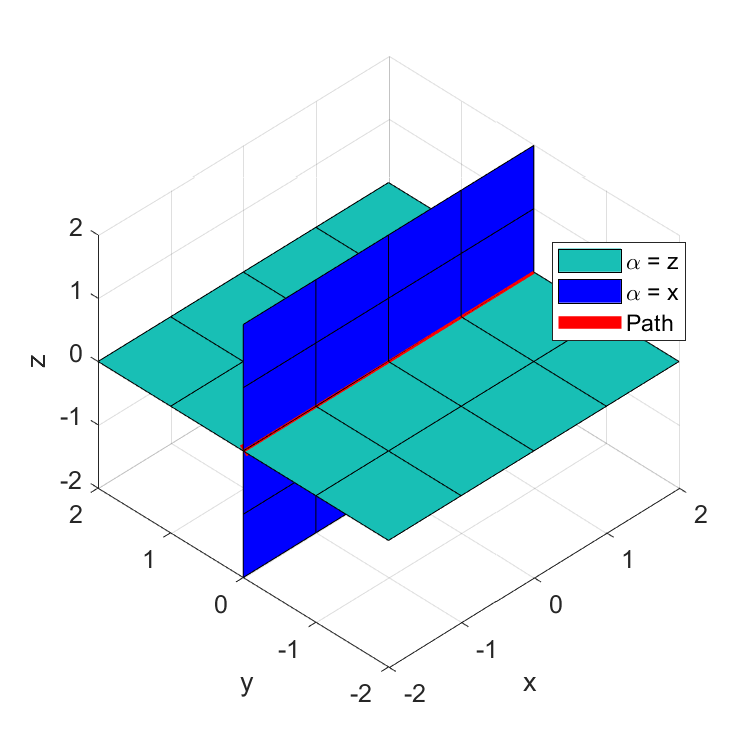
\includegraphics[width=7cm] {Figures/planeIntersection}}
		\subfigure []{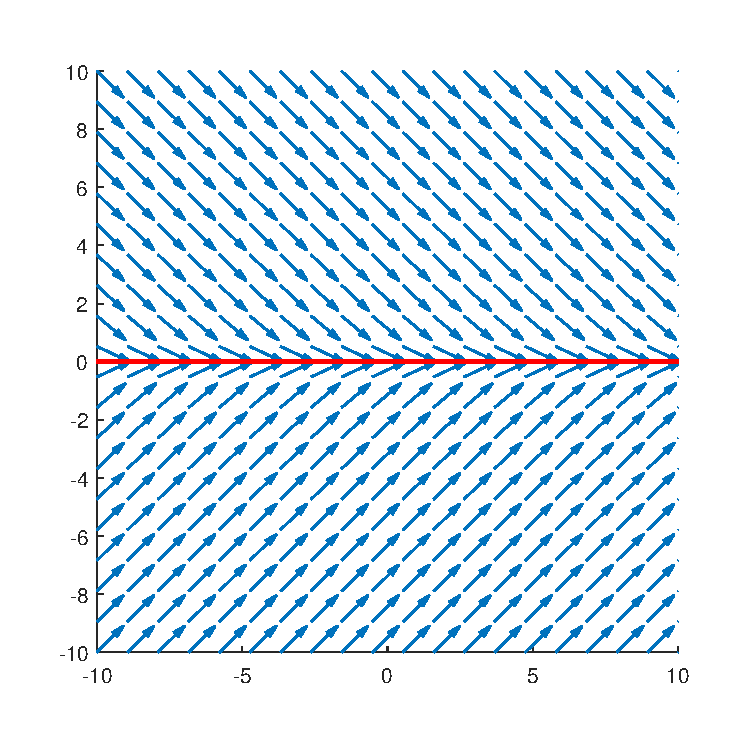
\includegraphics[width=7cm] {Figures/lineConvCirc}}
		\hspace*{0mm}
	\end{subfigmatrix}
	\caption{GVF converging and circulating straight path}
	\label{fig:GVFLine}
\end{figure} 



A GVF for converging and circulating a circular path can be produced by intersecting a plane and a cylinder $(\alpha_1 = z,\alpha_2 = x^2+y^2-r^2)$.
\begin{figure}[H]
	\begin{subfigmatrix}{2}% number of columns
		\centering	
		\subfigure []{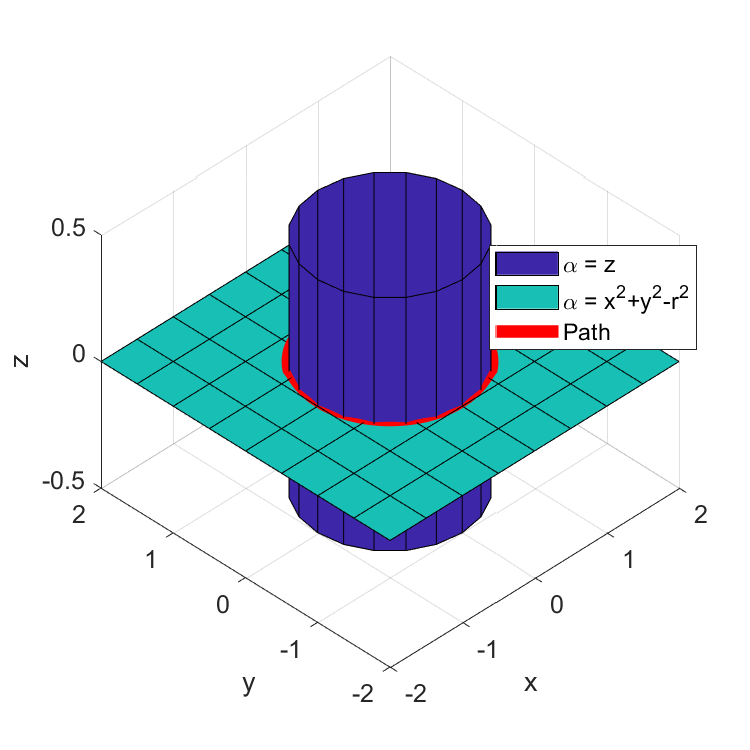
\includegraphics[width=7cm] {Figures/cylinderIntersection}}
		\subfigure []{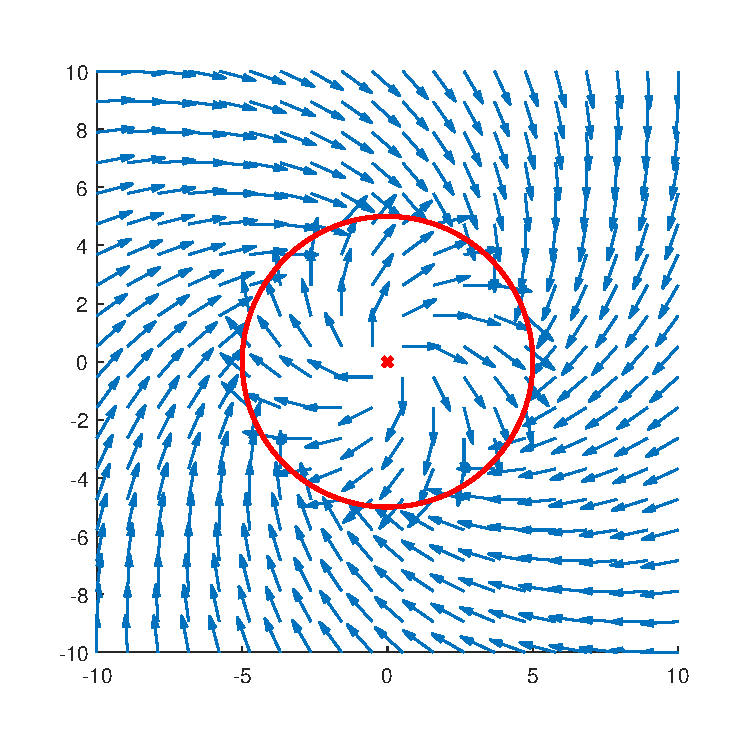
\includegraphics[width=7cm] {Figures/circConvCirc}}
		\hspace*{0mm}
	\end{subfigmatrix}
	\caption{GVF converging and circulating circular path}
	\label{fig:GVFLine}
\end{figure}

%The Goncalves method produces an \textit{n}-dimensional vector field that converges and circulates a static or time-varying path defined by \textit{(n-1)} implicit surfaces ($\alpha_i:\mathbb{R}^n\rightarrow\mathbb{R} | i=1,...,n-1$). The surface functions can represent any shape as long as they satisfy the two conditions that $1)$ they are positive definite and $2)$ have bounded derivatives. Consider the space with dimensions in set \textbf{q}:


GVF was compared against LVP in a standoff tracking scenario in [Wilhelm] where a fixed wing UAV was tasked with with loitering around a moving ground target while avoiding static obstacles.  A circular time-varying attractive vector field was attached to a moving ground target. Static circular repulsive vector fields centered at the obstacles and weighted by hyperbolic tangent decay functions were summed with the attractive circular field to produce a target loitering and obstacle avoidance guidance. The performance of Lyapunov \cite{frew_cooperative_2007} and gradient vector field \cite{goncalves_artificial_2009,goncalves_circulation_2010,goncalves_vector_2010} were compared for their cross track error with respect to the loiter circle. Gradient vector field had favorable performance due to compensation for a time-varying vector field. The gradient vector field technique also has the benefit of decoupled weighting parameters for convergence, circulation, and time-varying terms, allowing for easy modification of field behavior. \\

Decay functions for avoidance fields using GVF were investigated in [Zhu] for obstacles present on a straight path. When summing attractive and repulsive vector fields there is the possibility of guidance singularities, where magnitude and direction are equal and opposite. The presence of singularities were not addressed in [Wilhelm] and [Zhu], mentioned briefly in \cite{nelson_cooperative_2005} and observed in \cite{panagou_motion_2014}. For fixed wing UAVs the lack of guidance may prevent the UAV from avoiding an obstacle, while multi-rotor UAVs may end up in a trap situation. Singularities may be present at any location where a goal field and obstacle field are of equal strength. \\


\subsection{Dubins Vehicle}
Dubin's vehicle's position $\overrightarrow{X}$ at time $t$ is calculated from the integral of the velocity vector $\overrightarrow{U}$. The vehicle has a constant velocity magnitude $u_{uav}$ at a heading $\theta$. The rate at which $\theta$ changes with respect to time is based on limitations of the craft itself. 

\begin{equation}
\label{uavVelocity}
\overrightarrow{U}(t) = u_{uav} \begin{bmatrix}
cos(\theta(t)) \\
sin(\theta(t))
\end{bmatrix}
\end{equation}


\begin{equation}
\label{uavPosition}
\overrightarrow{X}(t) = \overrightarrow{U}dt + \overrightarrow{X}(t-1)
\end{equation}


\begin{equation}
\label{turnRate}
\dot{\theta} \leq 20 deg/s
\end{equation}




\section{methods}
Overview of methods \\
Construction of guidance for desired path \\
Construction of avoidance guidance \\
Path following and obstacle avoidance guidance \\
Singularity detection \\
Selection of vf parameters for optimized obstacle avoidance \\

\subsection{Path Following with GVF}
Path following guidance for a planar UAV at position $(x,y)$ for a time invariant line is achieved by summing together convergence $\overrightarrow{V}_{conv}$ and circulation $\overrightarrow{V}_{circ}$ terms shown in Equation \ref{eq:convAndCircOnly}.


where the plane defined by implicit surface function $\alpha_1$ is at angle $\delta$ and plane $\alpha_2$ is at constant height of $Z = 1$ shown in Equations \ref{eq:pathFunction} and \ref{eq:pathFunctionZ} respectively.


\begin{equation}
\label{eq:pathFunction}
\alpha_1 = cos(\delta)x + sin(\delta)y
\end{equation}

\begin{equation}
\label{eq:pathFunctionZ}
\alpha_2 = z
\end{equation}

The gradient $\nabla$ of the potential function $V$ is shown in Equation \ref{eq:potentialFunctionGrad}.

\begin{equation}
\label{eq:potentialFunctionGrad}
\nabla V = -\frac{1}{2(\sqrt{\cos^2(\delta) x^2+2\cos(\delta)\sin(\delta) xy +\sin^2 (\delta) y^2})} \begin{bmatrix}
2x\cos^2(\delta) + 2\cos(\delta)\sin(\delta) y \\
2y\sin^2(\delta) + 2\cos(\delta)\sin(\delta) x \\
2
\end{bmatrix}
\end{equation}

Circulation is calculated by the cross product of the surface function gradients, shown in Equation \ref{eq:circStraightPath} and \ref{eq:circStraightPat2}.



\begin{equation}
\label{eq:circStraightPat2}
\overrightarrow{V}_{circ} = \begin{bmatrix}
sin(\theta) \\
-cos(\theta) \\
0
\end{bmatrix}
\end{equation}

Guidance for a path at angle $\delta = 0$ and equal parts circulation and convergence weights $G=H=1$ is shown in Figure \ref{fig:straightpath} below.

\begin{figure}[H]
	\centering
	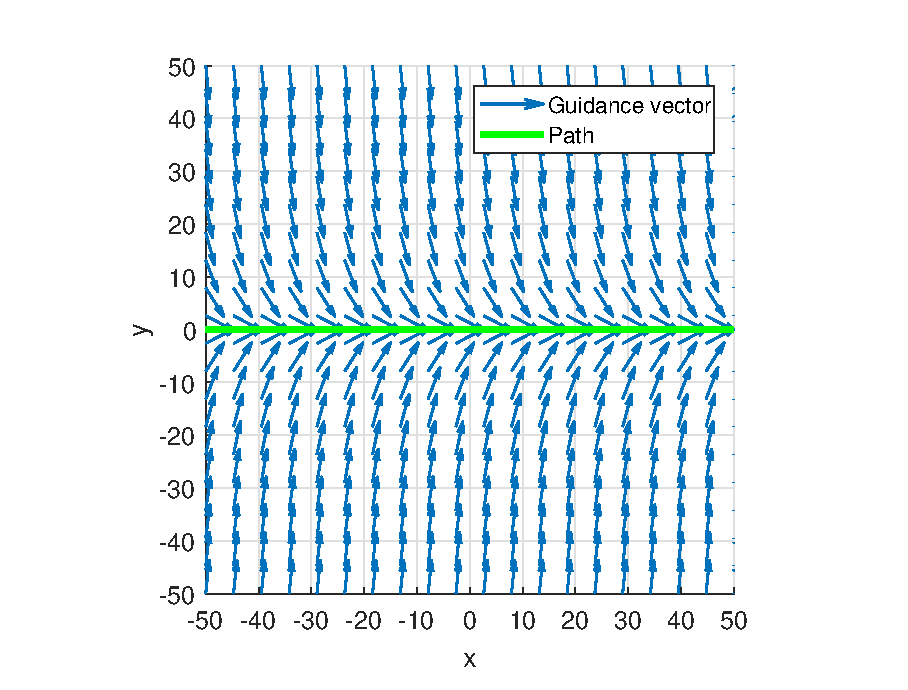
\includegraphics[width=0.7\linewidth]{Figures/methods/straightPath}
	\caption{}
	\label{fig:straightpath}
\end{figure}



\subsection{Avoidance}

Constructing a repulsive vector field for avoidance using the GVF method starts with constructing a vector field that converges and circulates a circular path. A GVF that converges and circulates a circular path is constructed with the implicit functions of a cylinder of radius $r$ centered at $(x_c,y_c)$ and a level plane of constant height $Z$, shown in Equations \ref{eq:alphaCylinder} and \ref{eq:alphaPlane} below.

\begin{equation}\label{eq:alphaCylinder}
\alpha_1 = (x-x_c)^2 + (y-y_c)^2-r^2
\end{equation}

\begin{equation}\label{eq:alphaPlane}
\alpha_2 = z
\end{equation}

Convergence is determined by the gradient of the potential function \ref{eq:potentialFunctionGrad}, which when simplified evaluates to

\begin{equation}
\overrightarrow{V}_{conv} = A\overrightarrow{B}
\end{equation}

where


\begin{equation}
A = \dfrac{-1}{\sqrt{\bar{x}^4+\bar{y}^4+2\bar{x}^2\bar{y}^2-2r^2\bar{x}^2-2r^2\bar{y}^2+r^2+z^2}}
\end{equation}

and

\begin{equation}
\overrightarrow{B} = \begin{bmatrix} 2\bar{x}^3+2\bar{x}\bar{y}^2-2r^2\bar{x} \\ 2\bar{y}^3+2\bar{x}^2\bar{y}-2r^2\bar{y} \\z \end{bmatrix}
\end{equation}.




\begin{equation}
\bar{x} = x - x_c
\end{equation}
\begin{equation}
\bar{y} = y - y_c
\end{equation}

Circulation is calculated from the cross product of each implicit surface functions gradient, which simplifies to

\begin{equation}\label{eq:vcirc_circle}
\overrightarrow{V}_{circ} =  \begin{bmatrix}  2(y-y_c) \\[6pt] -2(x-x_c) \\[6pt] 0\end{bmatrix}
\end{equation}

Guidance for avoiding a circular path with a large radius can be produced by setting the convergence weight $G=-1$ and circulation weight $H=0$, shown in Figure \ref{fig:largerepulsive}. Note that the vectors are normalized prior to applying decay to ensure the vector field strength is bounded.

\begin{figure}[H]
	\centering
	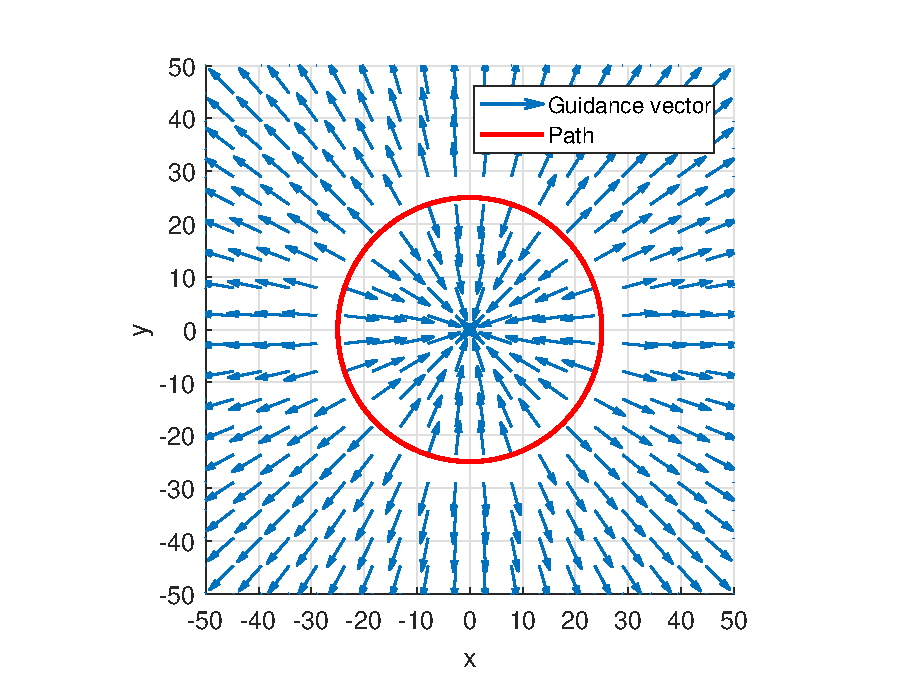
\includegraphics[width=0.7\linewidth]{Figures/methods/largeRepulsive}
	\caption{}
	\label{fig:largerepulsive}
\end{figure}

Note that inside of the path, vectors point towards the center of the circle which may produce a trap situation if the UAV ends up inside the radius. To prevent a trap situation inside of the circular path, the radius of the path can be reduced, as shown in Figure \ref{fig:normalizedrepulsive} where $r=0.01$.


\begin{figure}[H]
	\centering
	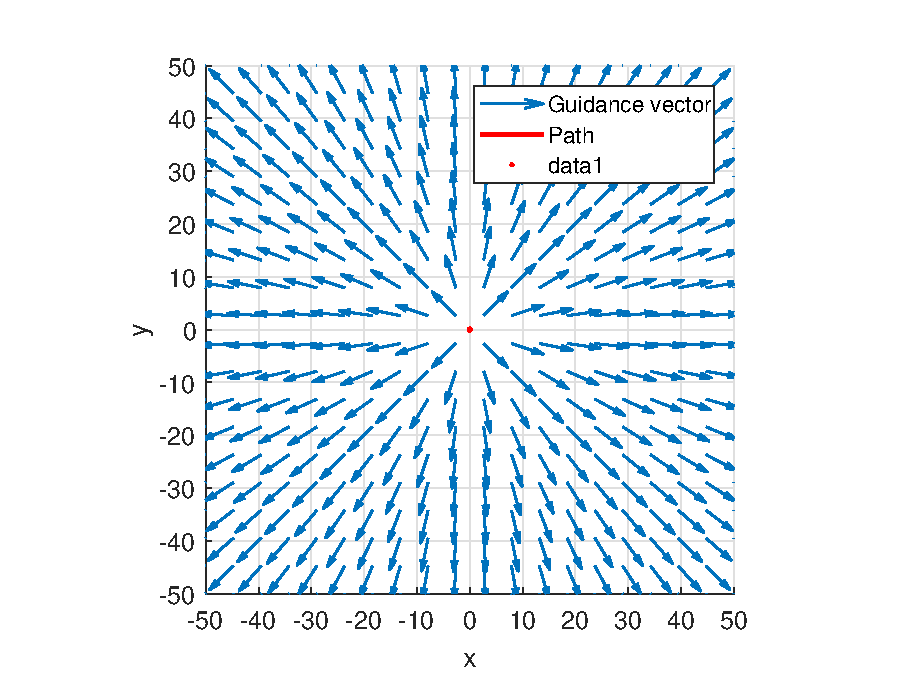
\includegraphics[width=0.7\linewidth]{Figures/methods/normalizedRepulsive}
	\caption{}
	\label{fig:normalizedrepulsive}
\end{figure}

To limit the influence of the repulsive field to a radius $R$, a decay function is applied prior to summing with the path following guidance. The decay strength $P$ is determined in \ref{eq:decay}, where $d$ is the euclidean distance, or range, between the UAV and the center of the obstacle, shown in Equation \ref{eq:range}. At a distance $d>R$ the decay strength $P$ is effectively zero, having virtual no influence on the total guidance. At a distance $d\leq R$, the field strength is bounded between $[0,2]$.


\begin{equation}
\label{eq:decay}
P = -\tanh \bigg( \frac{2\pi d}{R}-\pi\bigg)+1
\end{equation}

\begin{equation}
\label{eq:range}
d = \sqrt{ \bar{x}^2+\bar{y}^2}
\end{equation}

Applying the decay function with a decay edge radius $R = 35$ to the GVF shown in figure \ref{fig:normalizedrepulsive}, results in the field shown in Figure \ref{fig:decayapplied}.


%\begin{figure}[H]
%	\centering
%	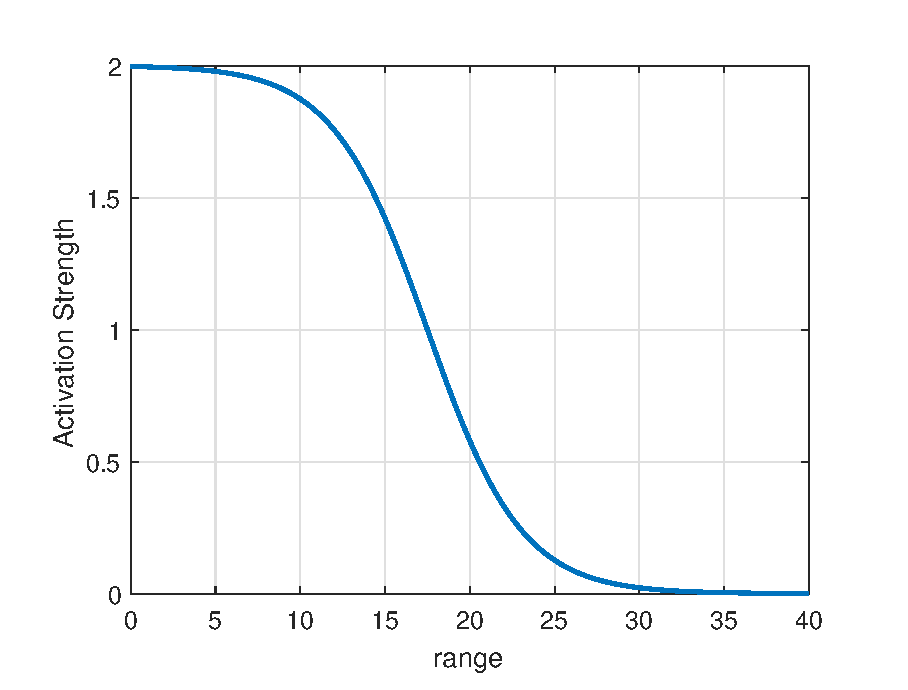
\includegraphics[width=0.7\linewidth]{Figures/methods/tanH}
%	\caption{}
%	\label{fig:tanh}
%\end{figure}



\begin{figure}[H]
	\centering
	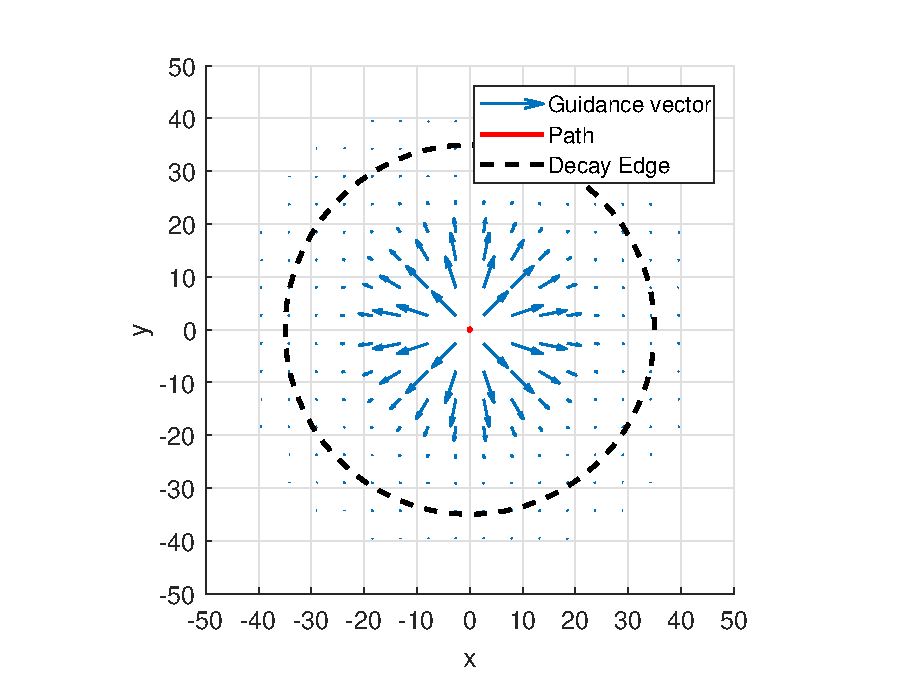
\includegraphics[width=0.7\linewidth]{Figures/methods/decayApplied}
	\caption{}
	\label{fig:decayapplied}
\end{figure}

%\begin{figure}[H]
%	\centering
%	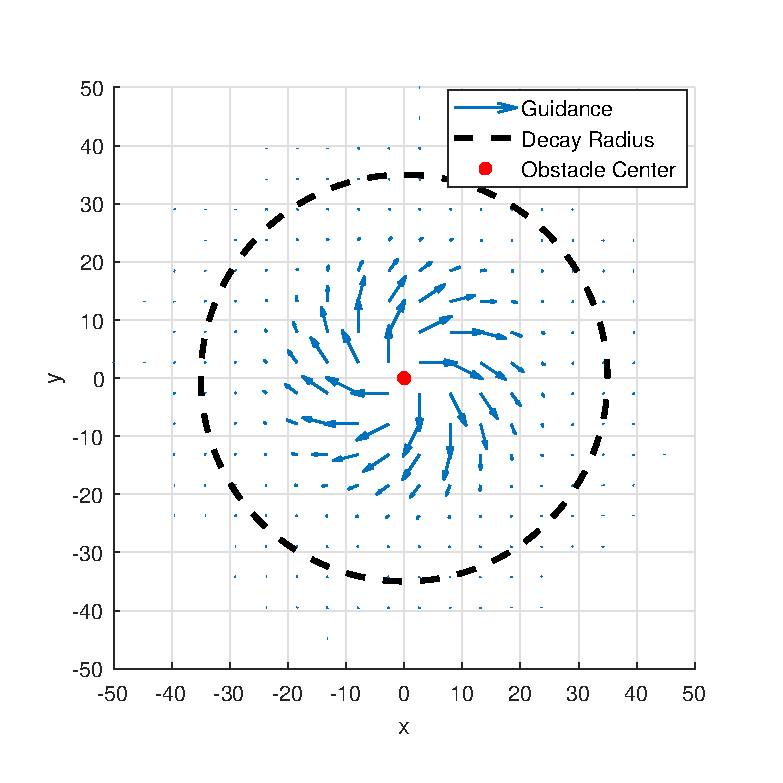
\includegraphics[width=0.7\linewidth]{Figures/methods/decayAppliedCirculation}
%	\caption{}
%	\label{fig:decayappliedcirculation}
%\end{figure}

Summing together the path following field with an obstacle centered on the path results in the guidance $\overrightarrow{V}_G$ shown in Figure \ref{fig:summedquiver}.

\begin{equation}
\label{eq:singularityCondition}
\overrightarrow{V}_g = \overrightarrow{V}_{path} + P\overrightarrow{V}_{obst}
\end{equation}




\begin{figure}[H]
	\centering
	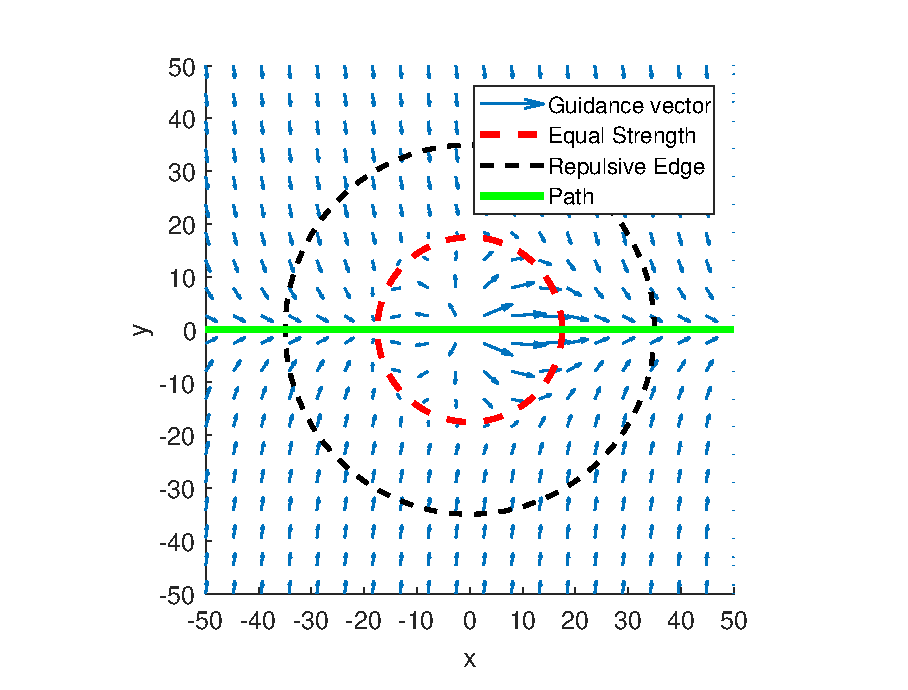
\includegraphics[width=0.7\linewidth]{Figures/methods/summedQuiver}
	\caption{}
	\label{fig:summedquiver}
\end{figure}










\subsection{Singularity Detection}
\begin{equation}
\label{eq:singularityCondition}
||\overrightarrow{V}_g || = 0
\end{equation}

Summing GVFs together may lead to small regions where the vector magnitude is near or equal to zero. Singularities are expected to exist where two summed fields have equal strength. The location of the singularities can be found by determining where the magnitude of the resulting guidance is equal to zero.


Plotting the magnitude of the summed field near the obstacle shows a well that descends into several local minimums called singularities, shown in Figure \ref{fig:summedmagnitudesurf}.


\begin{figure}[H]
	\centering
	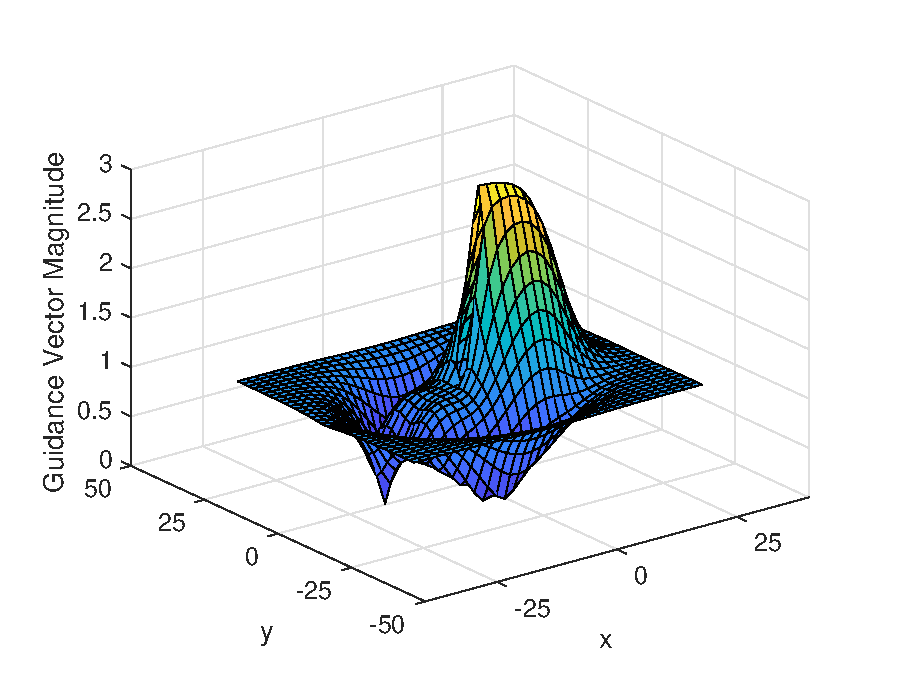
\includegraphics[width=0.7\linewidth]{Figures/methods/summedMagnitudeSurf}
	\caption{}
	\label{fig:summedmagnitudesurf}
\end{figure}

%Before using vector field guidance it is beneficial to know if singularities exist, where they are, and if the UAV will encounter them during flight. Singularities are expected to exist where two summed fields have equal strength. The location of the singularities can be found by determining where the magnitude of the resulting guidance is equal to zero.
 Multiple singularities or near zero guidance regions may exist, so several initial conditions must be evaluated to increase the probability of detection. With the path and obstacle field shown in \ref{fig:summedquiver}, several initial conditions evenly spaced were evaluated both inside and outside of the equal strength circle. Note how only points left of the obstacle were evaluated since this region is where attractive and repulsive vectors oppose each other, therefore it is where singularities are expected. Both inside and outside initial conditions determine the location of the singularities. 

\begin{figure}[H]
	\begin{subfigmatrix}{2}% number of columns
		\centering	
		\subfigure []{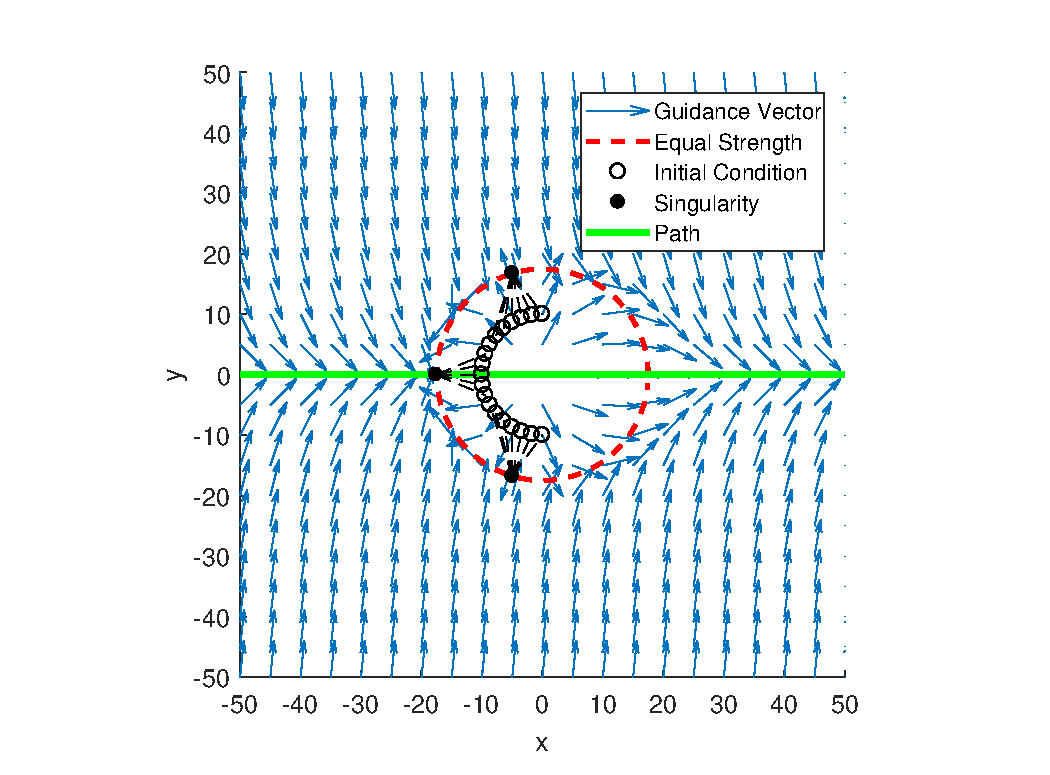
\includegraphics[trim=70 0 70 0,clip,width=8cm] {Figures/methods/noCircSingularityR10}}
		\subfigure []{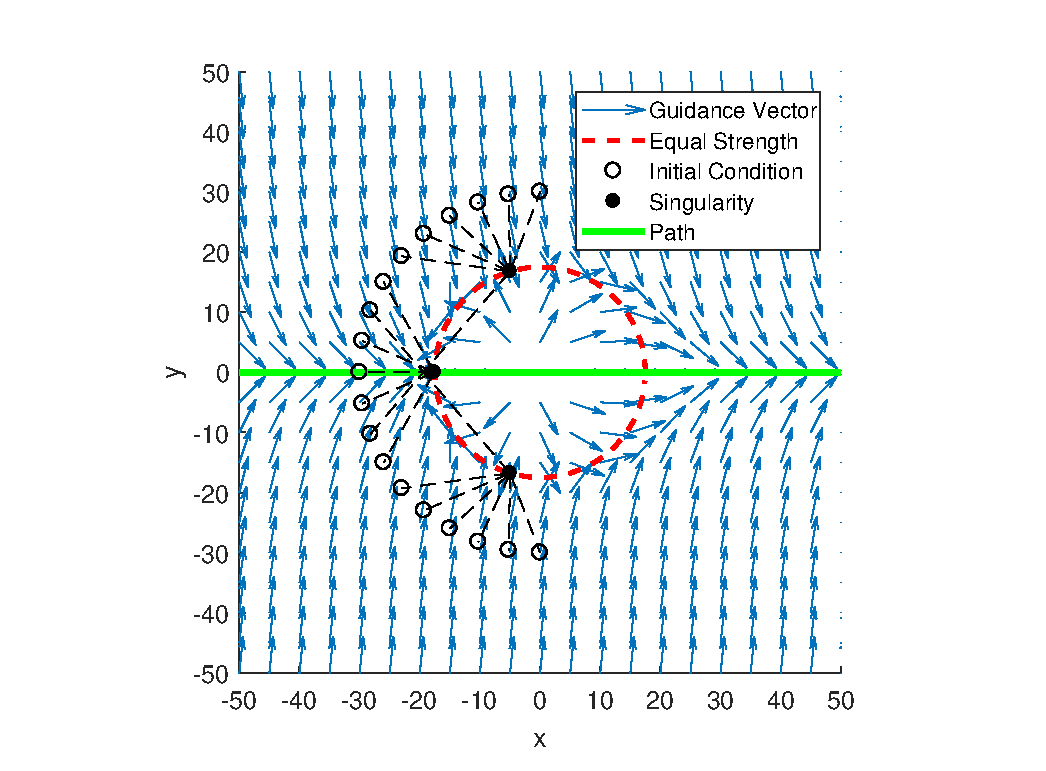
\includegraphics[trim=70 0 70 0,clip,width=8cm] {Figures/methods/noCircSingularityR30}}
		\hspace*{0mm}
	\end{subfigmatrix}
	\caption{GVF converging and circulating circular path}
	\label{fig:noCircSingularityDetection}
\end{figure}


%\begin{figure}
%	\centering
%	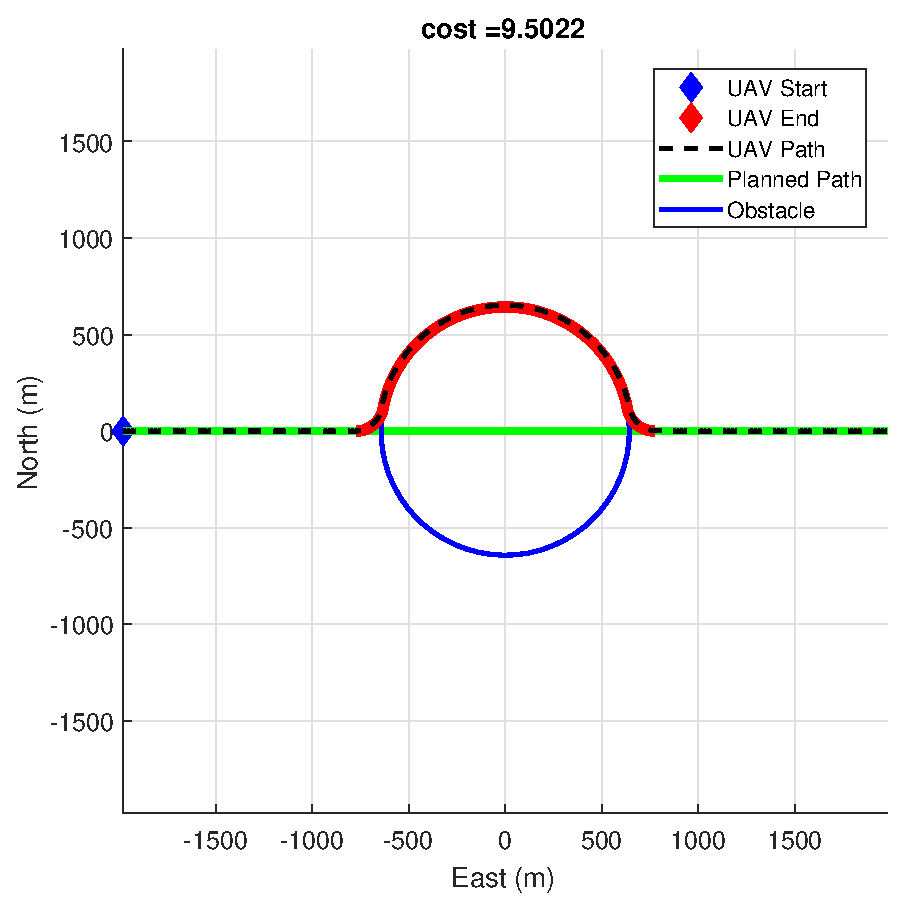
\includegraphics[width=0.7\linewidth]{Figures/semiFinalAlgorithm/Obsty0}
%	\caption{}
%	\label{fig:obsty0}
%\end{figure}
%\begin{figure}
%	\centering
%	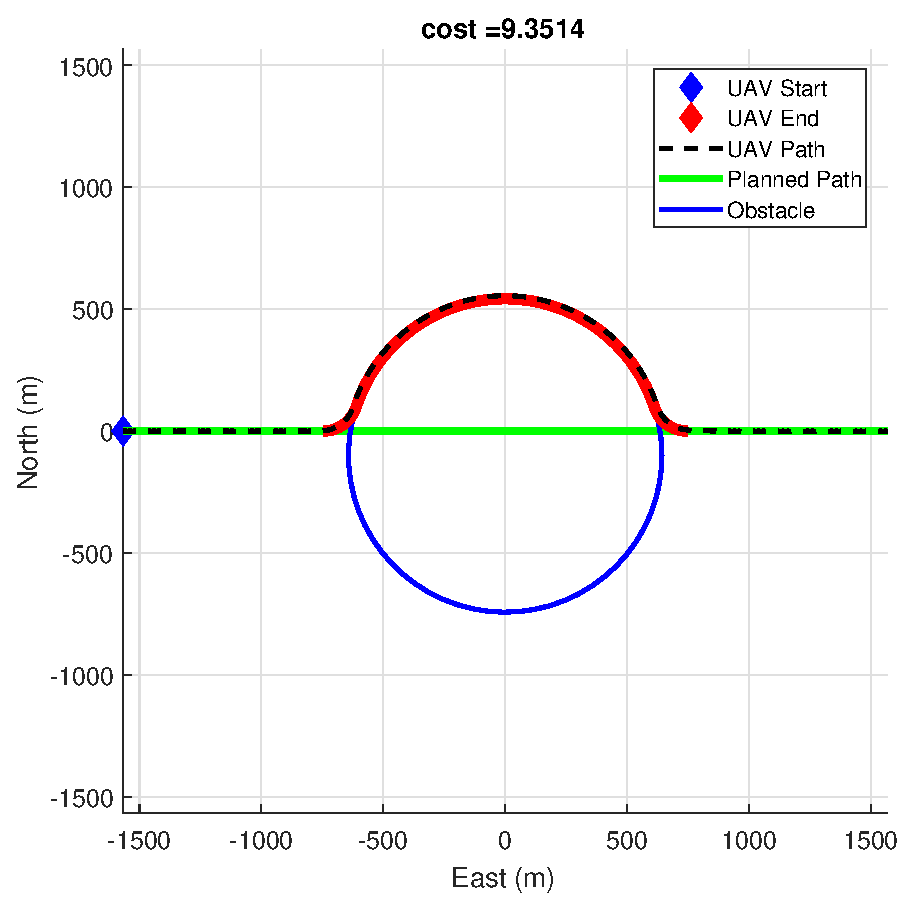
\includegraphics[width=0.7\linewidth]{Figures/semiFinalAlgorithm/Obsty-100}
%	\caption{}
%	\label{fig:obsty0}
%\end{figure}
%
%\begin{figure}
%	\centering
%	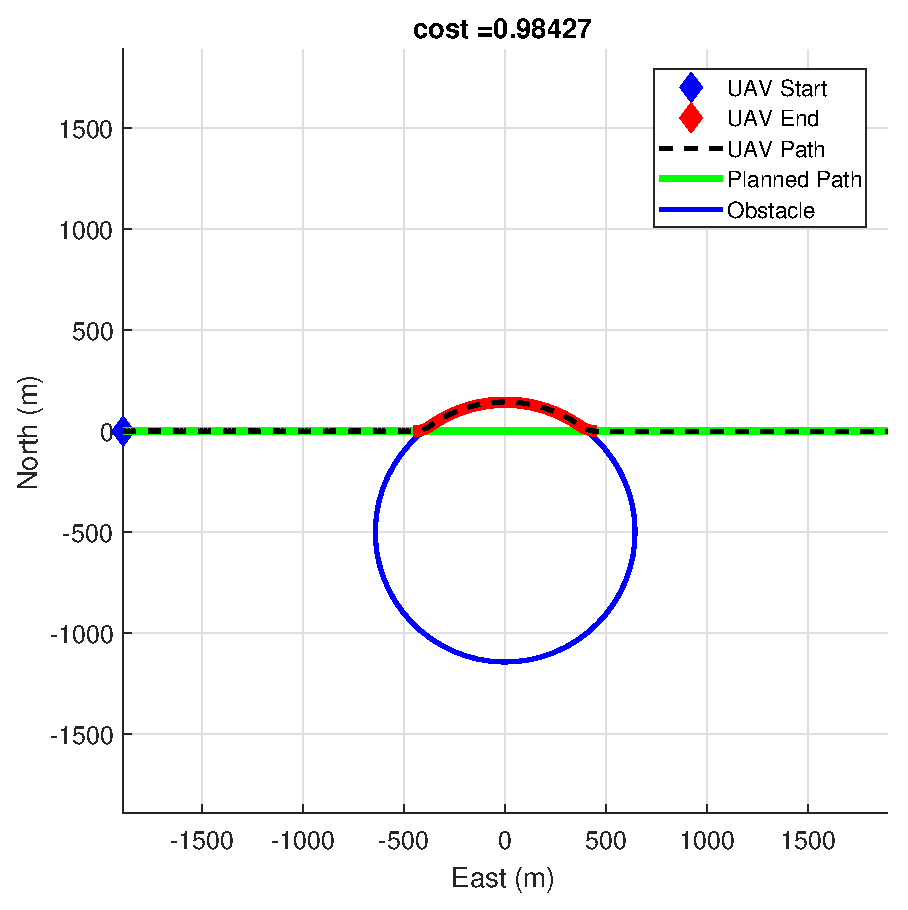
\includegraphics[width=0.7\linewidth]{Figures/semiFinalAlgorithm/Obsty-500}
%	\caption{}
%	\label{fig:obsty0}
%\end{figure}
%
%
%\begin{figure}
%	\centering
%	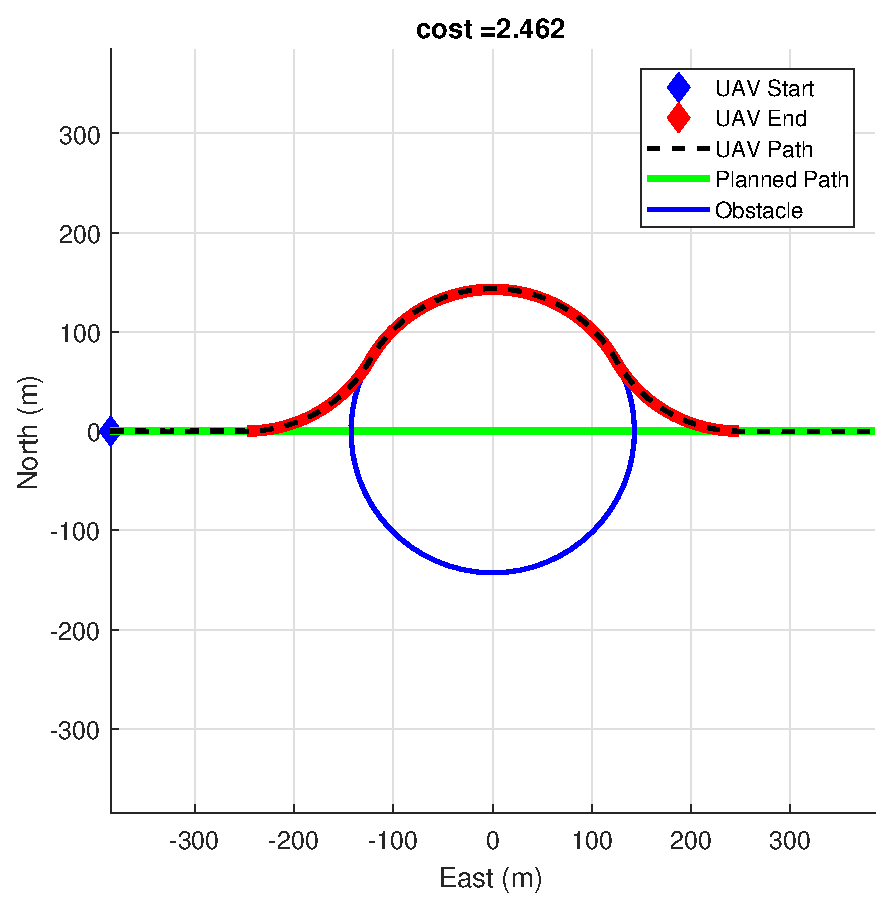
\includegraphics[width=0.7\linewidth]{Figures/semiFinalAlgorithm/ObstR142}
%	\caption{}
%	\label{fig:obsty0}
%\end{figure}
%
%\begin{figure}
%	\centering
%	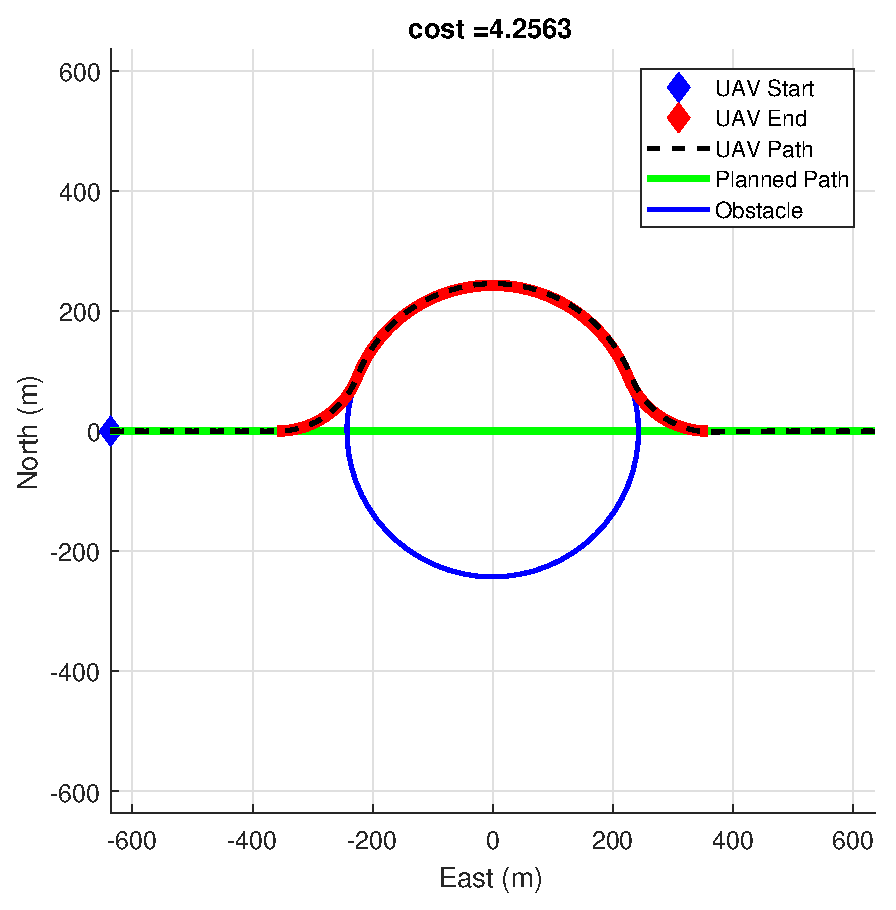
\includegraphics[width=0.7\linewidth]{Figures/semiFinalAlgorithm/ObstR242}
%	\caption{}
%	\label{fig:obsty0}
%\end{figure}
%
%\begin{figure}
%	\centering
%	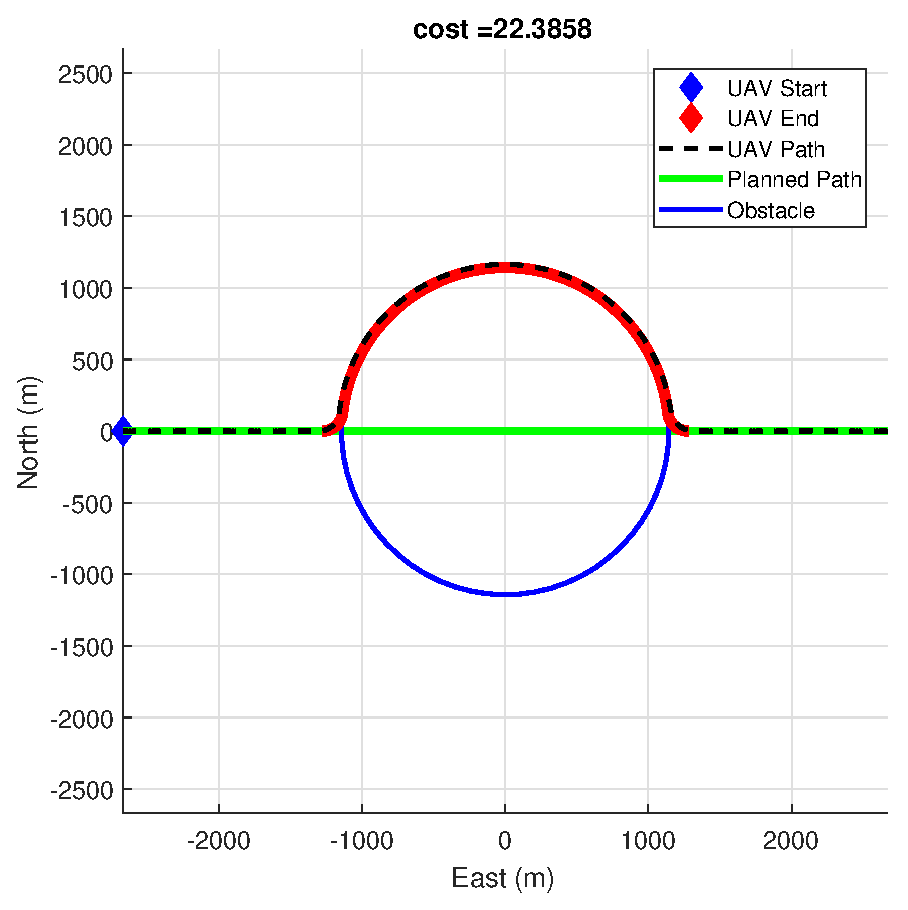
\includegraphics[width=0.7\linewidth]{Figures/semiFinalAlgorithm/ObstR1142}
%	\caption{}
%	\label{fig:obsty0}
%\end{figure}
%
%\begin{figure}
%	\centering
%	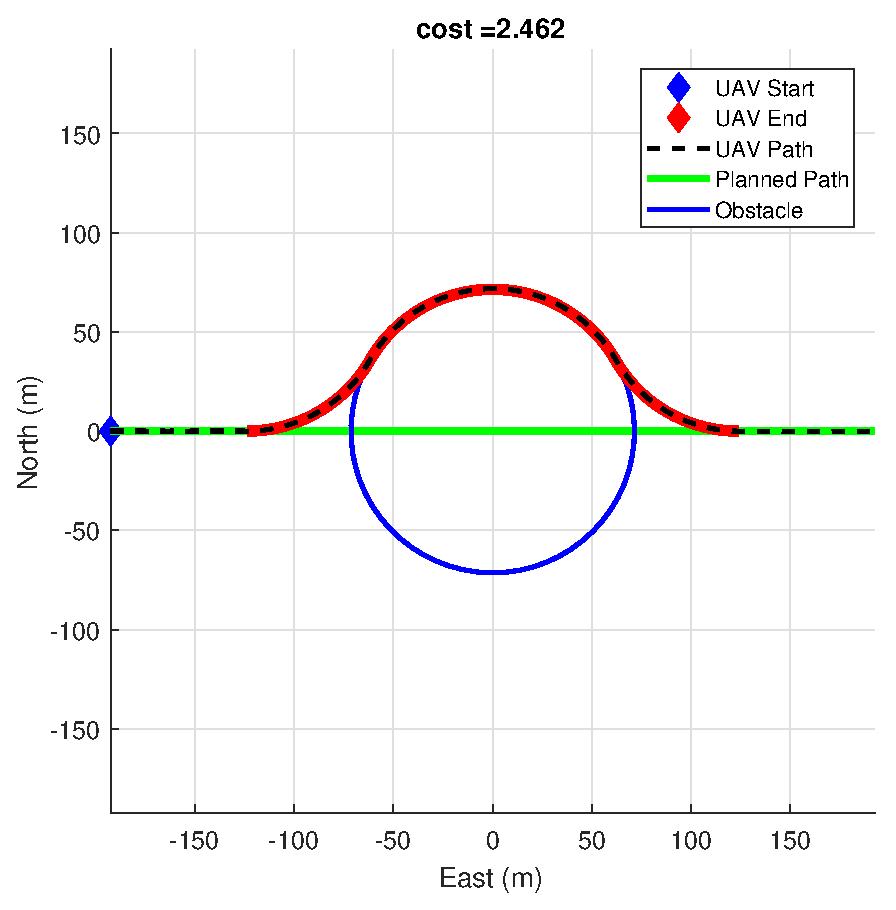
\includegraphics[width=0.7\linewidth]{Figures/semiFinalAlgorithm/Vs25}
%	\caption{}
%	\label{fig:obsty0}
%\end{figure}
%
%\begin{figure}
%	\centering
%	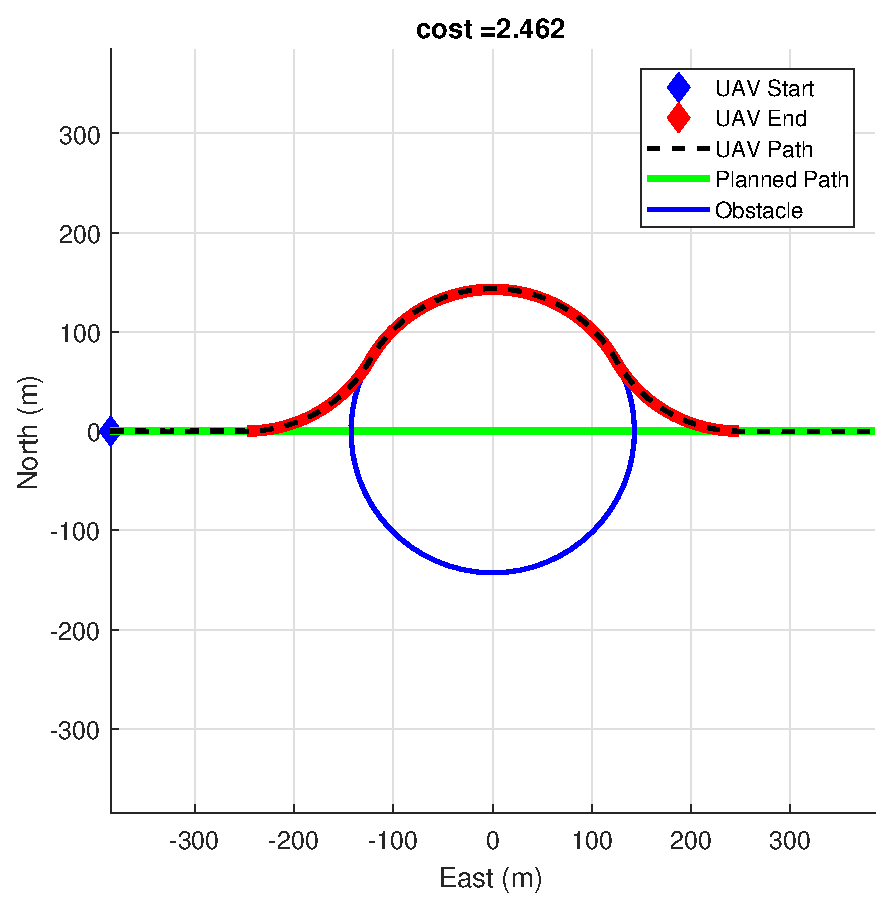
\includegraphics[width=0.7\linewidth]{Figures/semiFinalAlgorithm/Vs50}
%	\caption{}
%	\label{fig:obsty0}
%\end{figure}
%
%\begin{figure}
%	\centering
%	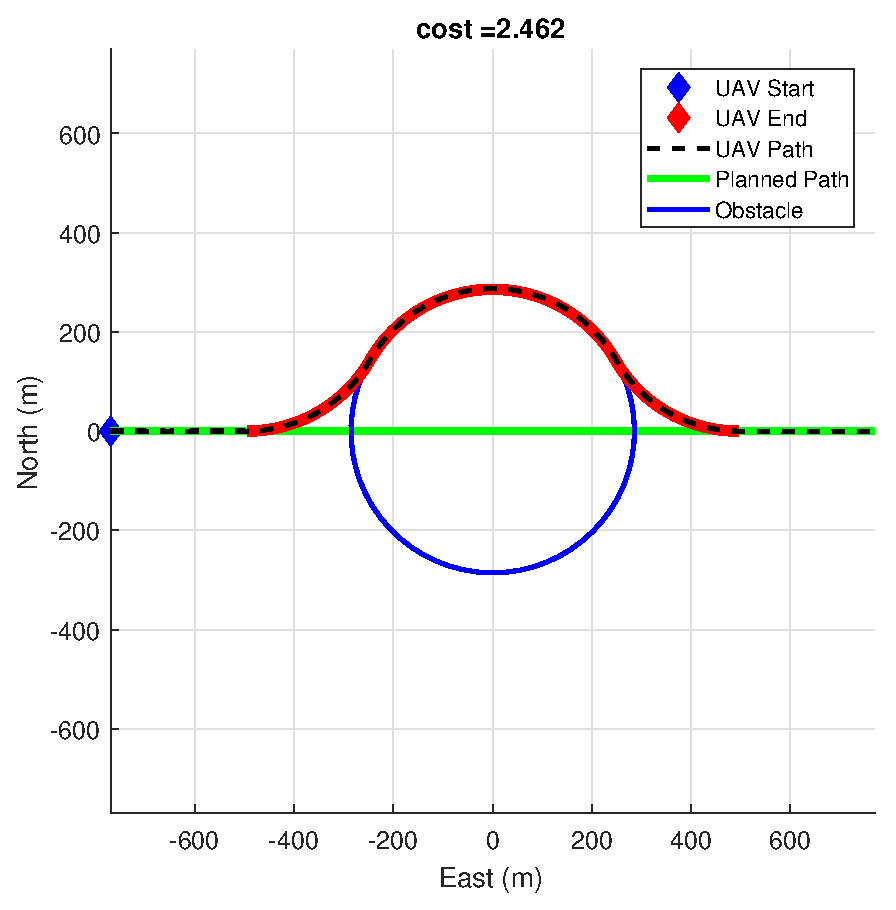
\includegraphics[width=0.7\linewidth]{Figures/semiFinalAlgorithm/Vs100}
%	\caption{}
%	\label{fig:obsty0}
%\end{figure}


















\subsection{Flight Envelope}
Evaluating a large number of initial conditions to improve the probability of finding singularities may be computationally expensive and may also find singularities the UAV may not encounter. Selecting a reduced set of initial conditions and to determine if the singularities exist where the UAV may fly, a flight envelope is determined for some time horizon $t_h$. Consider the UAV depicted in Figure \ref{fig:flightenvelope2} with a turn rate $\dot{\theta}$ and fixed speed $u$. 

\begin{figure}[H]
	\centering
	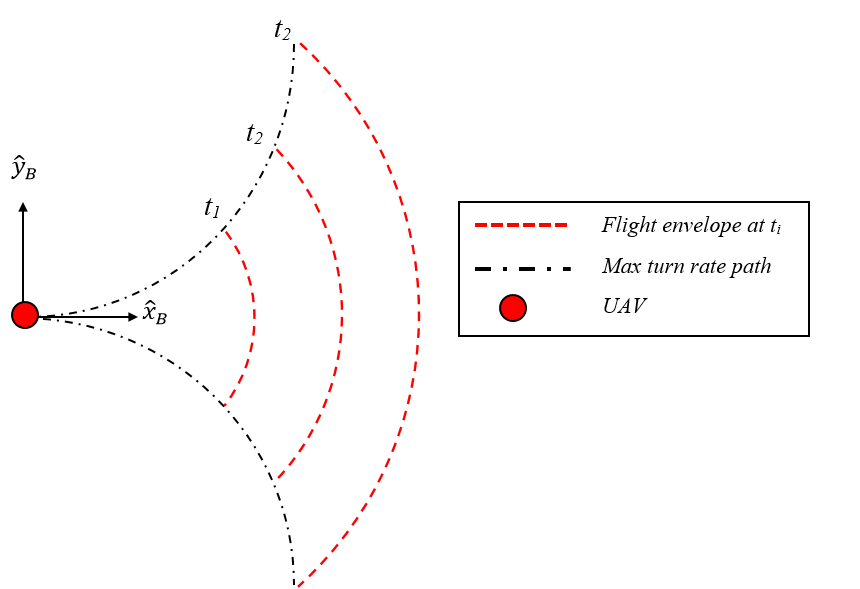
\includegraphics[width=0.7\linewidth]{Figures/methods/flightEnvelope2}
	\caption{}
	\label{fig:flightenvelope2}
\end{figure}

The flight envelope, or positions the UAV, at time $t_i$ with respect to the body frame is calculated in Equations \ref{eq:qx} and \ref{eq:qy}

\begin{equation}
\label{eq:qx}
q_x =  \frac{u}{\dot{\theta}} \sin(t_h \dot{\theta})
\end{equation}

\begin{equation}
\label{eq:qy}
q_y =  \frac{u}{\dot{\theta}} \big(1-\cos(t_h \dot{\theta})\big)
\end{equation}

It is convenient to represent points on the flight envelope in the global inertial frame. The flight envelope points $(q_x,q_y)$ can be expressed in vector form by finding the angle $\phi$ with respect to the body frame $\hat{x}_b$ axis and the vector magnitude $q$ shown in equations \ref{eq:qphi} and \ref{eq:qMag} respectively.




\begin{equation}
\label{eq:qphi}
\phi = \tan^{-1} \bigg( \frac{q_y}{q_x} \bigg)
\end{equation}

\begin{equation}
\label{eq:qMag}
q = \sqrt{q_x^2 +q_y^2}
\end{equation}



\begin{equation}
\label{eq:pos}
\overrightarrow{Q_b} = \begin{bmatrix}
	q\cos\phi \\
	q\sin\phi \\
	0
\end{bmatrix}
\end{equation}

To express the flight envelope in the global inertial frame, the position vector of the UAV $\overrightarrow{P}_0$ and $\theta$ are applied with a rotation matrix $R$, shown in Equations \ref{eq:pos}, \ref{eq:rotation}, and \ref{eq:qGlobal} below. 


\begin{figure}[H]
	\centering
	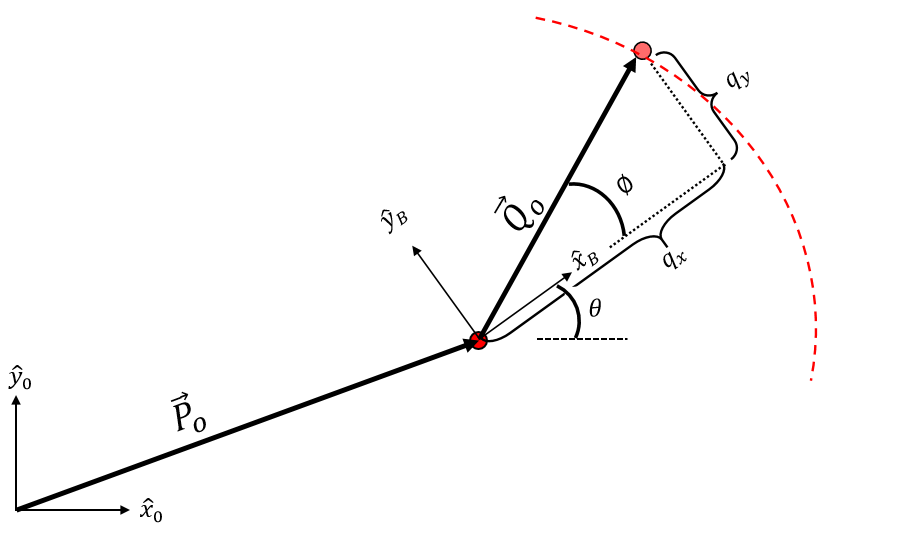
\includegraphics[width=0.7\linewidth]{Figures/methods/flightEnvelope}
	\caption{}
	\label{fig:flightenvelope}
\end{figure}


\begin{equation}
\label{eq:rotation}
\overrightarrow{P}_0 = \begin{bmatrix}
x & y & 0
\end{bmatrix}^T
\end{equation}


\begin{equation}
\label{eq:qGlobal}
   R=\begin{bmatrix}
	\cos(\theta) & -\sin(\theta) & 0 \\
	\sin(\theta) & \cos(\theta) & 0 \\
	0 & 0 & 1 \\
\end{bmatrix}
\end{equation}


\begin{equation}
\label{eq:pos}
\overrightarrow{Q}_0 = \overrightarrow{P_0} + R  \overrightarrow{Q_b}
\end{equation}


Initial conditions placed on the flight envelope will follow the magnitude gradient of the GVF guidance and locate any singularities it may encounter. When a singularity is found to exist inside or near a flight envelope the field can be modified to counteract it. 


\section{Simulations}
\begin{figure}
	\centering
	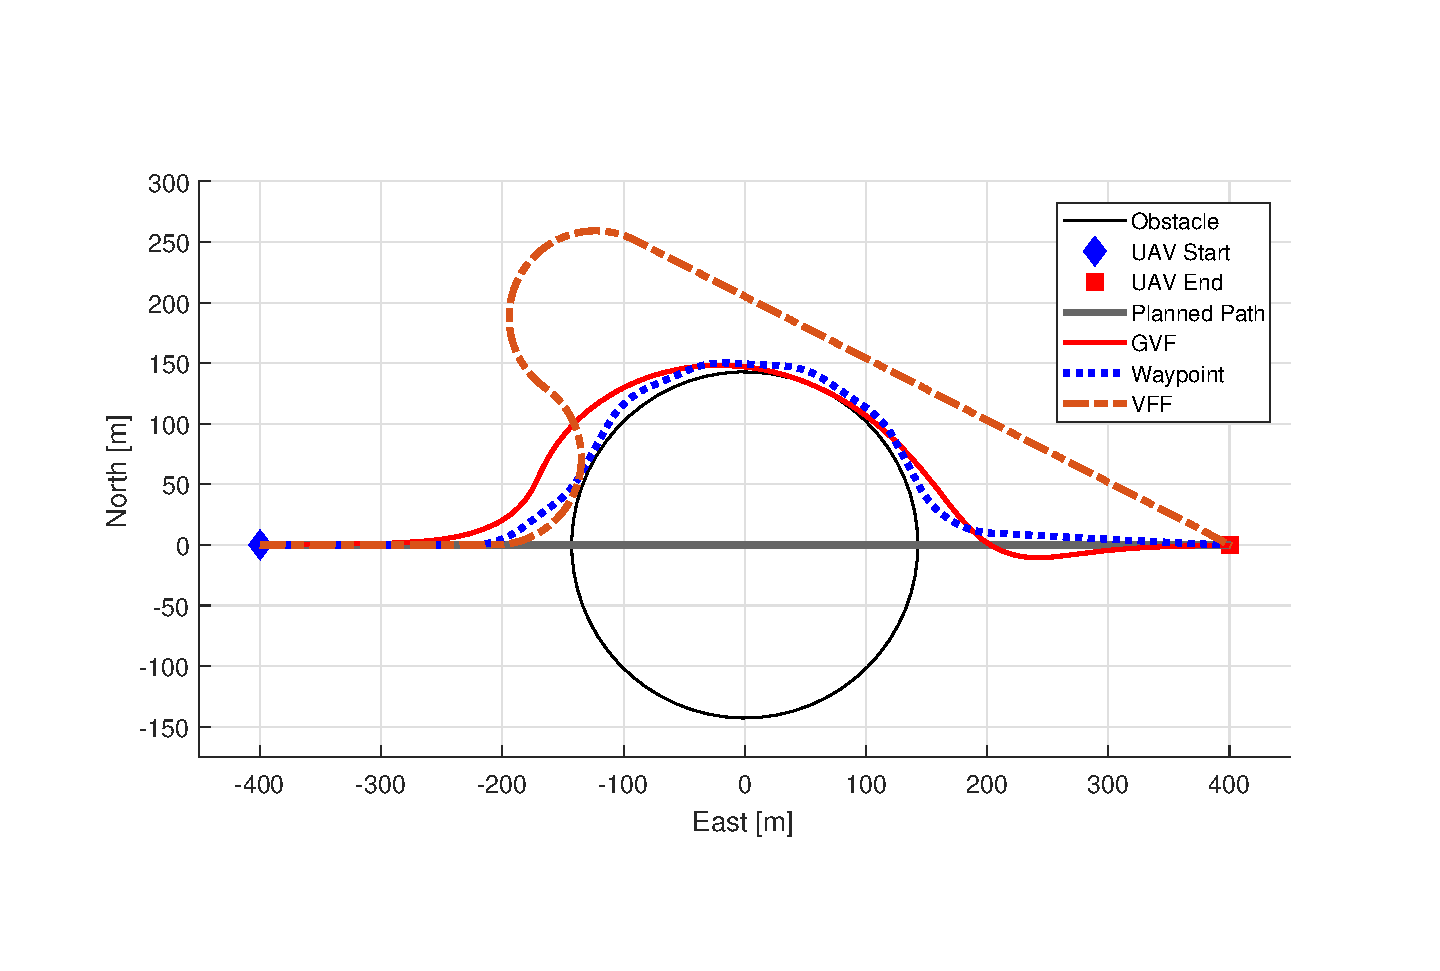
\includegraphics[width=0.7\linewidth]{Figures/Simulations/compareMethods}
	\caption{}
	\label{fig:comparemethods}
\end{figure}





\section{Conclusion}


\begin{tabular}{|c|c|c|}
	\hline 
	Method & Cost (-) & RMS Error (m) \\ 
	\hline 
	Waypoint & 16.34 & 16.75 \\ 
	\hline 
	VFF & 34.87 & 91.65 \\ 
	\hline 
	GVF & 13.79 & 1.65 \\ 
	\hline 
\end{tabular} 
\section*{Appendix}



\section*{Acknowledgments}

\bibliography{bib}

\end{document}
